%--------------------
% Packages
% -------------------
\documentclass[11pt,a4paper]{report}
%\usepackage{gentium}

\usepackage[
backend=biber,
style=nature,
sorting=ynt
]{biblatex}
\addbibresource{references.bib}

\usepackage[pdftex]{graphicx} % Required for including pictures
\usepackage[english, danish]{babel} % Swedish translations
\usepackage[pdftex,linkcolor=black,pdfborder={0 0 0}]{hyperref} % Format links for pdf
\usepackage{calc} % To reset the counter in the document after title page
\usepackage{enumitem} % Includes lists
\usepackage{caption}
\usepackage{subcaption}
\usepackage{xcolor}
\definecolor{LightGray}{gray}{0.9}
\usepackage{minted}
\setminted{bgcolor=LightGray, breaklines=true, fontsize=\footnotesize}

\frenchspacing % No double spacing between sentences
\linespread{1.2} % Set linespace
\usepackage[a4paper, lmargin=0.1666\paperwidth, rmargin=0.1666\paperwidth, tmargin=0.1111\paperheight, bmargin=0.1111\paperheight]{geometry} %margins
%\usepackage{parskip}
\usepackage{titling}
\newcommand{\subtitle}[1]{%
  \posttitle{%
    \par\end{center}
    \begin{center}\large#1\end{center}
    \vskip0.5em}%
}
\usepackage{booktabs}
\usepackage{todonotes}


\usepackage[all]{nowidow} % Tries to remove widows
\usepackage[protrusion=true,expansion=true]{microtype} % Improves typography, load after fontpackage is selected

% Define a utility function to write vector symbols in bold
\newcommand{\bm}[1]{\textbf{#1}}
\newcommand{\vecsym}[1]{\bm{#1}}
% And a matrix symbol
\newcommand{\matsym}[1]{\bm{#1}}
% And a tensor symbol
\newcommand{\tenssym}[1]{\bm{#1}}

\title{Ruling out the rulers}
\subtitle{Understanding and checking for bias in skin lesion classification models}
\author{Mikkel Bjørn Goldschmidt}

\usepackage{amsfonts}
\usepackage{amsmath}
\usepackage{amssymb}
%-----------------------
% Set pdf information and add title, fill in the fields
%-----------------------
\hypersetup{ 	
pdfsubject = {Medical image analysis, XAI},
pdftitle = {Ruling out the rulers},
pdfauthor = {Mikkel Bjørn Goldschmidt}
}

\renewcommand\sectionmark[1]{\markright{\thesection.\ #1}}

%-----------------------
% Begin document
%-----------------------
\begin{document}
\selectlanguage{english}
\maketitle

\tableofcontents
\pagebreak
\renewcommand{\chaptername}{Section} 
\begin{center}
\vspace*{\fill}
\begin{large}
    \textbf{Preface and Acknowledgements}
\end{large}

This project is written as my thesis for my bachelor's degree in Mathemathics and Technology at
the Danish Technical University.
It has been written at the Department of Applied Mathematics and Computer Science and supervised by
Professor Aasa Feragen and PhD-student Manxi Lin. 

I would like to acknowledge and give my warmest thanks both of them for all of their help and support.
Their quick and insightful feedback along the way got me through the research process and the writing of this report.



\end{center}
\vspace*{\fill}
\pagebreak
\vspace*{\fill}
\selectlanguage{english} 
\begin{abstract}
Deep learning models can be used to classify medical images.
This may be problematic, as models reportedly use confounding elements (elements
 in the images that are not supposed to be used in the classification),
in their predictions.
Multiple studies have been conducted to understand, demonstrate and
mitigate the effects of these elements.

This project investigates the impact of one example,
namely, rulers in images of skin lesions originally used by 
doctors to monitor lesion growth.
A close to state-of-the-art classification model is trained, and
using methods of other researchers as well as other methods,
it is concluded, that the model is not using these rulers.
Further, it is argued that other models trained on the same data,
are also unlikely to use the rulers in their predictions.
It is also seen that in general models trained with access to less
information around the lesions perform better, suggesting that
the confounding elements contained there are not necessary
for the models predictions.
Based on the difficulty of the research, it is recommended that
care is taken when making claims about the impact of a confounding 
element on a given model.

\end{abstract}
\vspace*{\fill}
\selectlanguage{danish} 
\begin{abstract}
Abstract på dansk
\end{abstract}
\selectlanguage{english}
\vspace*{\fill}

\renewcommand{\chaptername}{Section} 
\pagebreak
\chapter{Introduction}
Image analysis can be used in the diagnosis of diseases in different ways.
A lot of the data used for diagnosing come in the form of images.
Examples of these are MRI, CT, PET, ultrasound but also just plain images of body parts.
Understanding these images is often done using machine learning models in different forms.
In their nature, these models are not easy to understand and can therefore end up biased without
the model designer knowing it.

This project focuses on the HAM10000 dataset\cite{Tschandl_2018}, which contains images of skin lesions.
Doctors diagnose these lesions into different classes, some more dangerous than others.
The challenge on the HAM10000 dataset is to find a model that can predict the class of a given image.

\subsection{Biases in the data}
Many different models have been trained to diagnose lesions based on medical images.
These images are taken in a real world medical context, which can introduce unknown bias into the models.
It has even been reported that models trained on medical data where the lesions were masked out,
% THIS IS NOT TRUE! 73% percent refers to AUC not accuracy.
could reach an accuracy of $73\%$\cite{DeConstructing_Bias_on_Skin_Lesion_Datasets_2019}, indicating that there are other factors in the data, 
that can be used to classify the models than the actual lesion.
Some research has tried to introduce foreign object into the images,
and found that they changed the classification of the lesions \cite{Towards_Explainable_Classifiers_Using_the_Counterfactual_Approach_2019}.
These foreign objects included ruler markings, black frames and colored circles.

\section{The HAM10000 dataset}
The HAM10000 dataset contains 10015 images of skin lesions.
These images are a subset of the images from the ISIC dataset\cite{ISIC_Dataset_2018},
which collects images of skin lesions and hosts annual competitions for skin lesion diagnosis.
They are divided into seven classes as seen in the Table \ref{table:ham10000}.
A \textit{severity} has also been assigned each class.
These indicate if the lesion class benign, malignant or pre-malignant.
Malignant tumors are those where the cells are replicationg uncontrollably,
and there is a risk of these cells spreading to the rest of the body.
Beningn tumors can still hurt the patient, but are much less of a worry,
as they are not replicationg uncontrollably and hence do not lead to cancer.

\begin{table}[ht]
\begin{center}
\begin{tabular}{|c|c|c|c|c|c|c|}
\hline
Label    & Name                          & Severity      & Dataset prevalence \\ \hline
akiec    & Bowens disease                & pre-malignant & $3.27\%$           \\ \hline
nv       & Melanocytic nevi              & benign        & $66.94\%$          \\ \hline
mel      & Melanoma                      & malignant     & $11.11\%$          \\ \hline
bkl      & Benign keratosis-like lesions & benign        & $10.97\%$          \\ \hline
bcc      & Basal cell carcinoma          & malignant     & $5.13\%$           \\ \hline
vasc     & Vascular lesions              & benign        & $1.41\%$           \\ \hline
df       & Dermatofibroma                & benign        & $1.14\%$           \\ \hline
\end{tabular}
\end{center}

\caption{Overview of the HAM10000 dataset.}
\label{table:ham10000}
\end{table}

\subsection{State of the art models}
Due to the public nature of the dataset, many different models have been trained on it.
As of the time of writing, the best performing model published in a scientific paper,
reaches an accuracy of $93.4\%$\cite{datta2021soft}.

\subsection{Confounding elements in the data} \label{sec:confounding}
The dataset contains images of skin lesions, which are taken in a real world medical context.
In this context doctors might introduce foreign objects into the images,
to help in the treatment of the patient.
Examples of these can be seen on Figure \ref{fig:confounding_objects}.

\begin{figure}[ht]
    \begin{center}
        \begin{subfigure}[b]{0.3\textwidth}
            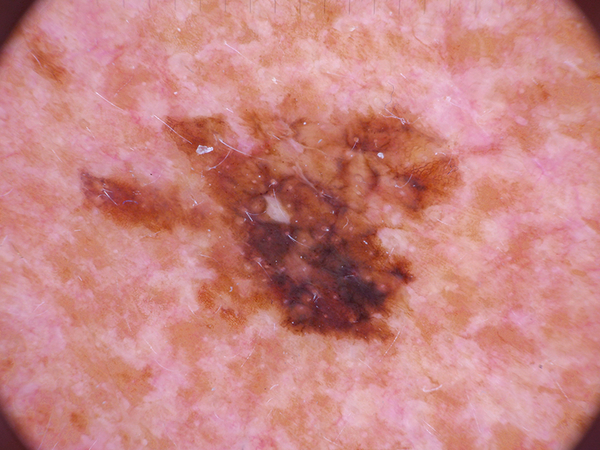
\includegraphics[width=\textwidth]{./images/ISIC_0024310.jpg}
            \caption{Image with black frame}
        \end{subfigure}
        \begin{subfigure}[b]{0.3\textwidth}
            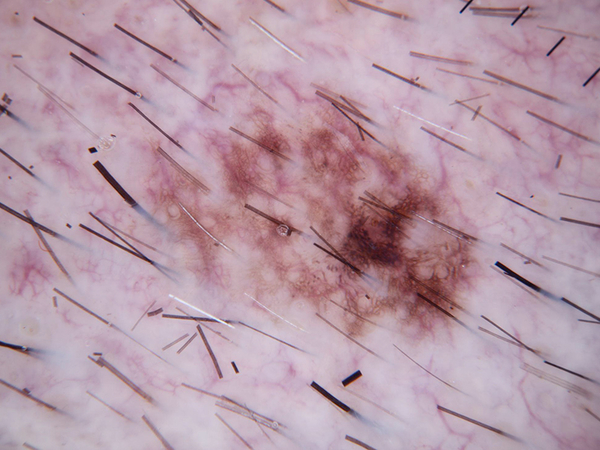
\includegraphics[width=\textwidth]{./images/ISIC_0024420.jpg}
            \caption{Image with ruler}
        \end{subfigure}
        \begin{subfigure}[b]{0.3\textwidth}
            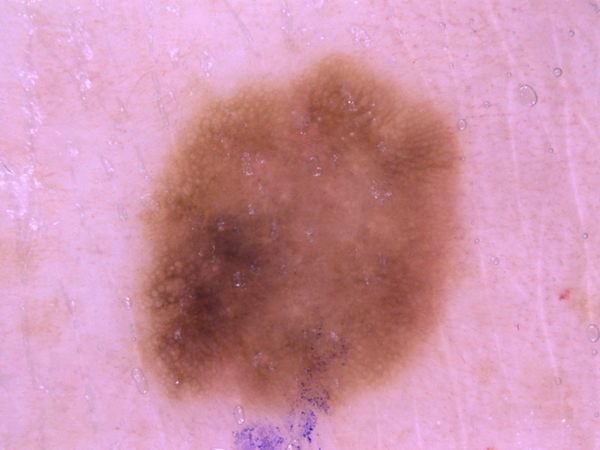
\includegraphics[width=\textwidth]{./images/ISIC_0027514.jpg}
            \caption{Image with blue ink}
        \end{subfigure}
    \end{center}
    \caption{Images with different confounding objects}
    \label{fig:confounding_objects}
\end{figure}

Labeling some of these confounding objects, we see that the rulers occur way more often than the others with a prevalence of roughly $17\%$ (See Table \ref{table:confounding_objects}).
Due to this higher prevalence, the study done in this project will focus on the ruler markings over the other confounding objects.

\begin{table}
    \centering
    \begin{tabular}{|l|r|}
        % confounding_objects.ipynb
        \hline 
        Confounder &  Prevalence \\ \hline
        ruler   &  0.171842 \\ \hline
        sticker &  0.000100 \\ \hline
        ink     &  0.003495 \\ \hline
    \end{tabular}
    \caption{Dataset prevalence of confounding objects}
    \label{table:confounding_objects}
\end{table}

\subsection{Correlation between confounding elements and HAM10000 labels}
On Figure \ref{fig:ruler_vs_dx} indications of correlations between the ruler markings and the HAM10000 labels can be seen.

\begin{figure}[ht]

\centering
\includegraphics[width=0.8\textwidth]{./build/confounder_label_correlation/confusion_matrix_seaborn.png}
\caption{Confusion matrix of rulers vs. class in the HAM10000 dataset - normalized over the x-axis.}
\label{fig:ruler_vs_dx}
\end{figure}

The two benign classes \textit{mel} and \textit{bkl} are both over represented on pictures with ruler markings copared to those without.
In general almost every class except the biggest \textit{nv} class is over represented.
The hypothesis that the presence of rulers in the images is correlated with the HAM10000, can be confirmed by a $\chi^2$-contingency test.
The null hypothesis of this test is that the presence of rulers in the images is not correlated with the HAM10000 labels.
The test value is 
    $\input{build/confounder_label_correlation/chi2.txt}$
on a test with
    $\input{build/confounder_label_correlation/dof.txt}$
degrees of freedom, resulting in a $p$-value of 
    $\input{build/confounder_label_correlation/p.txt}$
which is obviously significant.


\chapter{Related work}
\section{Debiasing Skin Lesion Datasets and Model. Not So Fast}\label{sec:debias-not-so-fast}
In their paper
''Debiasing Skin Lesion Datasets and Model. Not So Fast''
Bissoto, Alceu and Valle look into debiasing models trained on
skin lesion images \cite{debias-not-so-fast}.
They go through $7$ different artifacts in the images that could
be confounding elements, and try state-of-the-art methods to
make them disregard the artifacts.
These include the rulers, that is the focus of this report.
The paper makes several claims about biases that occur in
their skin lesion classification models.
Their focus is the removal of these bias, but the relevance to this project is that they
make claims about their models actually being biased.

\subsection{Arguments that the model is using the artifacts}
The researchers trained multiple different models to detect if the
images contained malignant or benign lesions.
Note that this classification is a simplified version of the classes
that is used in this report, as they only focus on whether a lesion is malignant or benign.
The researchers used the RESNET-18 architecture, as the basis for all their models.
They then utilize that the architecture is set up in a way where first a set of features
are extracted from the images using convolutional layers, and then fed into a fully connected layer. 
An outline of this is shown on Figure \ref{fig:resnet-outline}.

\begin{center}
    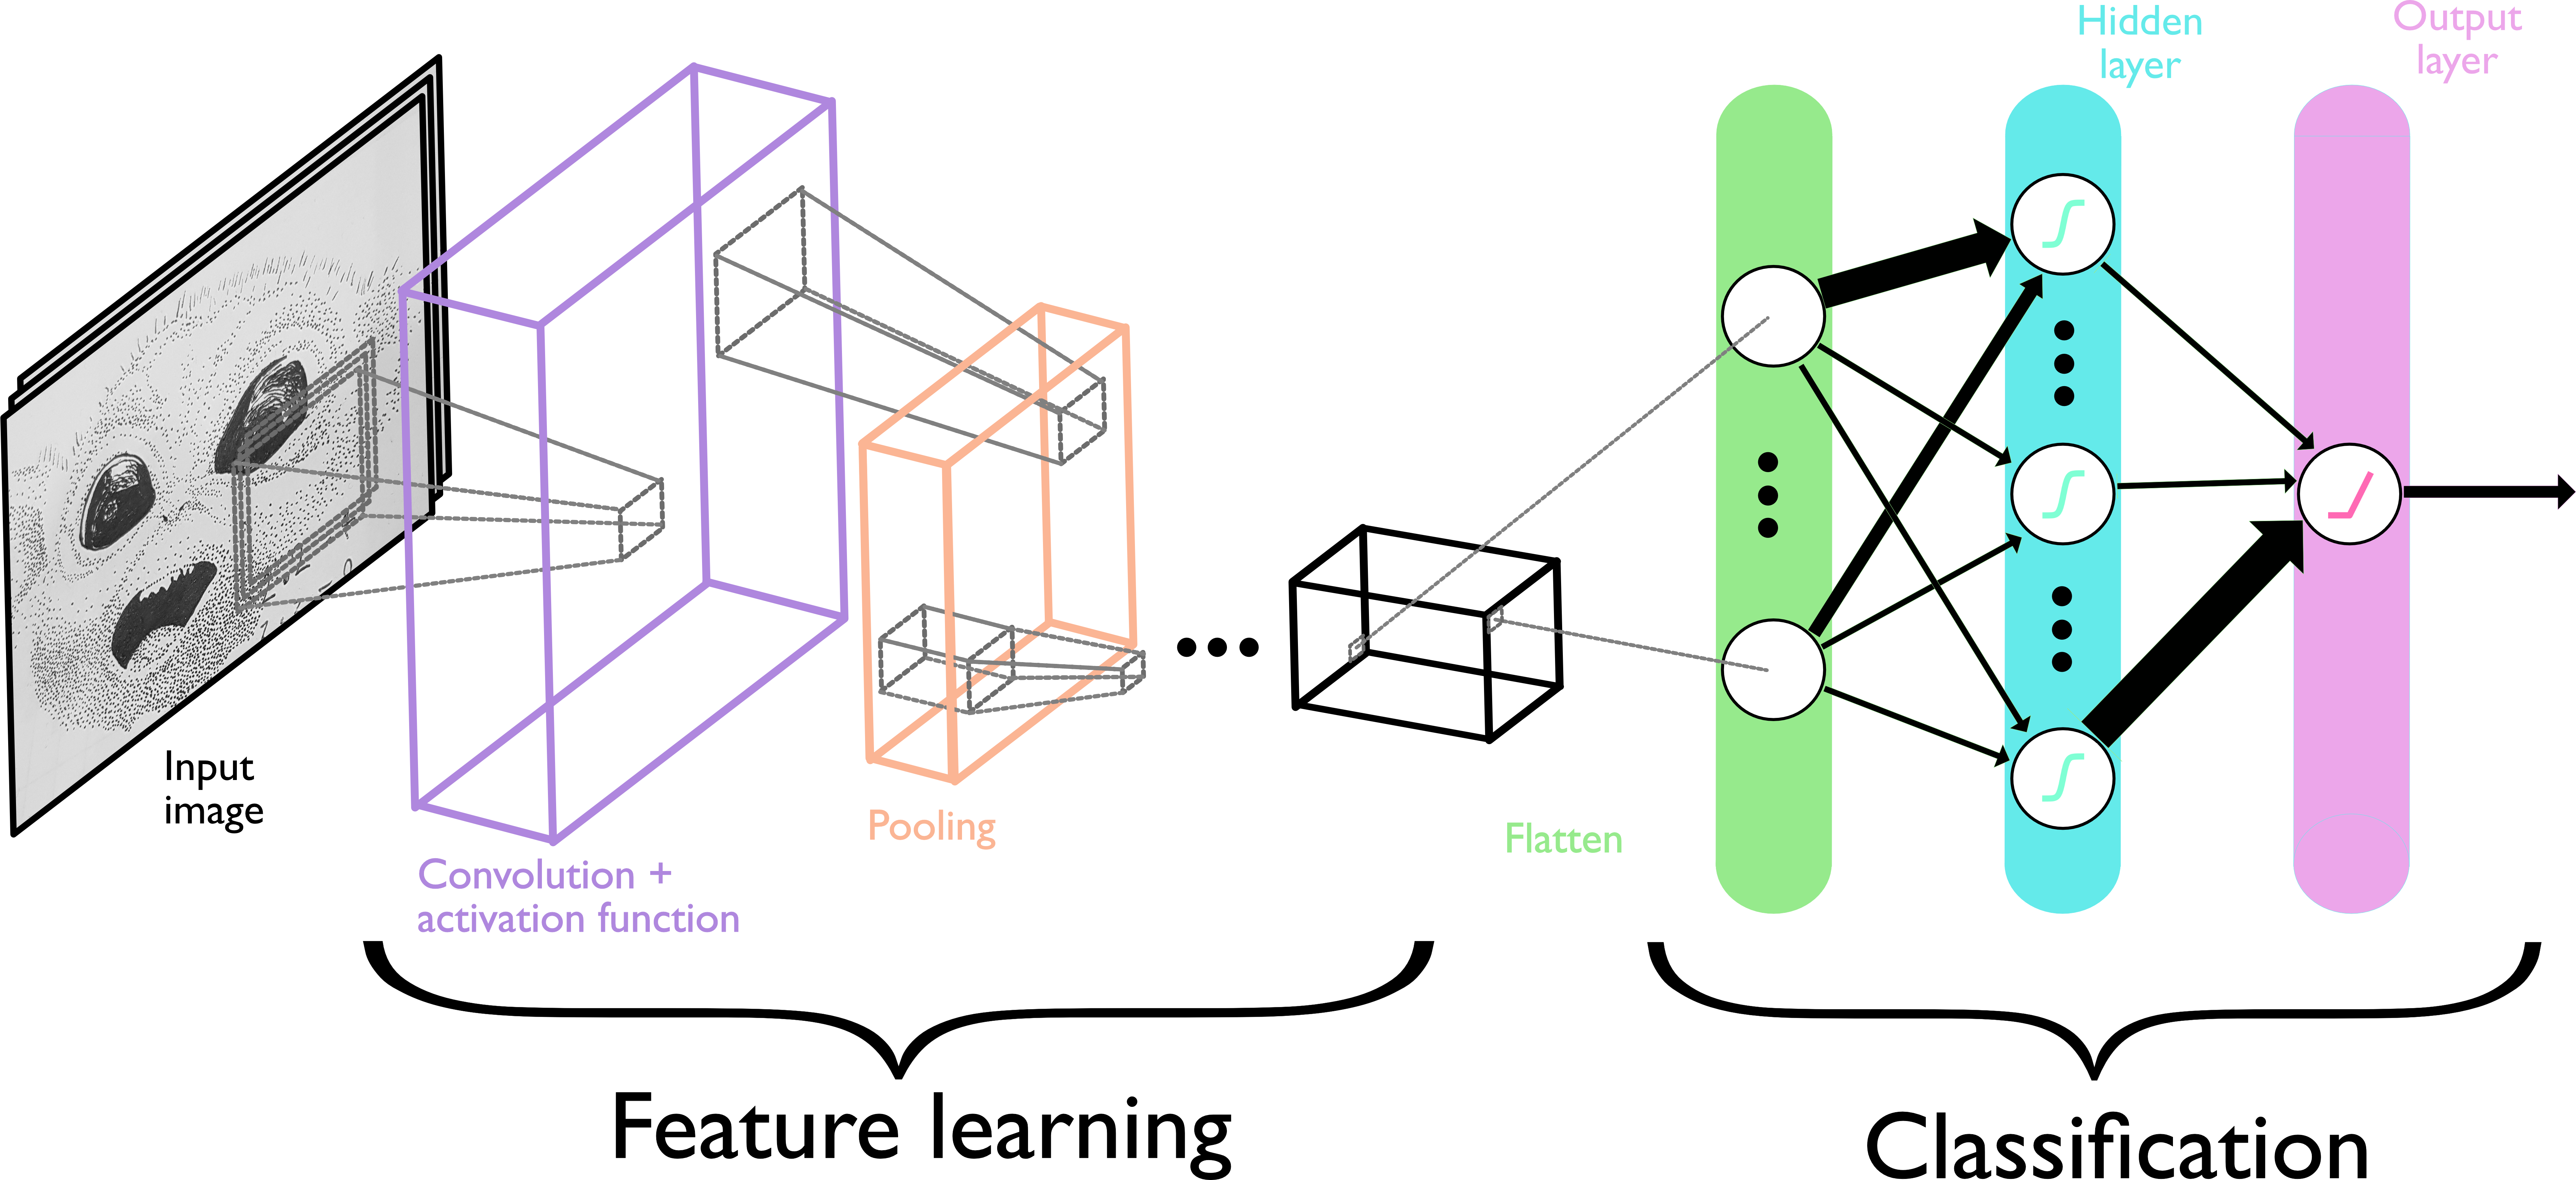
\includegraphics[width=0.9\textwidth]{images/ConvNet_V2.png}
    \captionof{figure}{A simplified view of how CNNs in general are structured with
                       convolutional layers first that extract features and fully connected layers
                       at the end to handle the classification.
                       This figure is borrowed from my wonderful writing partners \cite{alex-og-felix}.
    }
    \label{fig:resnet-outline}
\end{center}

As shown in the figure, the convolutional layer outputs a tensor (for definition of tensors, see Section \ref{sec:tensor}).
This tensor can then be converted into a vector, which can be interpreted as a feature vector for the image.
Intuitively, two images with \textit{similar} elements in the image should have a similar feature vector.
Utilizing this idea, the researchers calculate these vectors for the entire test dataset.
They then find that there is a relatively small euclidean distance between the feature vectors of images
that contain the same artifacts.
They show this by finding the nearest neighbors (with the distance measure between images being the euclidean distance between their feature vectors)
of different images artifact, and find that these neighbors often contain the same artifacts.
Their results are shown in Figure \ref{fig:not-so-fast-artifact-query}.


\begin{center}
    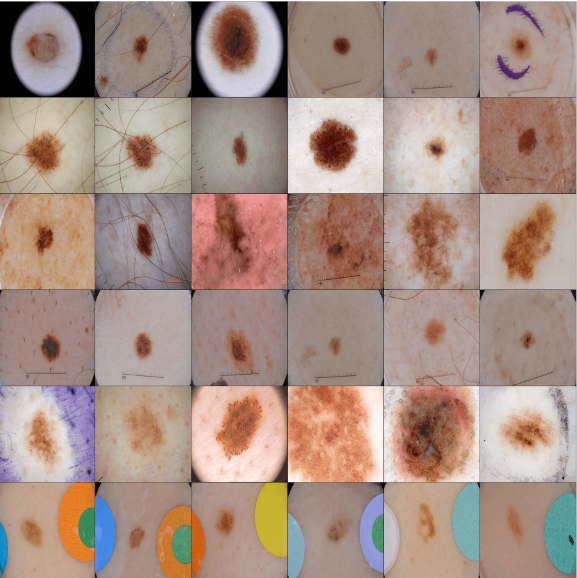
\includegraphics[width=0.4\textwidth]{images/not-so-fast-artifact-query.png}
    \captionof{figure}[Figure 4.a from \cite{debias-not-so-fast}]{
            Figure 4.a from \cite{debias-not-so-fast}, original description: \textit{Grid showing image similarity according to the features extracted by our classification model. The first column
            of each grid is the query, and the remaining columns are ranked according to euclidean distance of the images features.
            We selected queries carefully to show different artifacts.
            In sequence, dark corners, hair, gel border, ruler, ink markings and patches}}
    \label{fig:not-so-fast-artifact-query}
\end{center}

From the fact that the feature vectors of the images with the same artifacts are relatively small,
they conclude that the model is biased towards the artifacts - since the features it extracts seem to contain information about the artifacts.
The paper then goes on to examining how to mitigate these biases, but this is not relevant to this report.
\pagebreak
\section{Interpretations are useful: Penalizing Explanations to Align Neural Networks with Prior Knowledge}
In their paper \textit{Interpretations are useful: Penalizing Explanations to Align Neural Networks with Prior Knowledge}\cite{interps-are-useful},
Rieger, Singh, Murdoch and Yu propose a method to penalize a model during training,
if it does not align with the prior knowledge of the dataset (for instance that a ruler shouldn't be used to classify a benign tumor).
To show examples of their method, they (among other things) train a model on the ISIC dataset \cite{ISIC_Dataset_2018}.

Here, they are able to use saliency maps (see section \ref{sec:saliency_maps}) to see, that the model is using rulers to classify benign lesions.
In Figure \ref{fig:interps-are-useful-saliency-maps}, their figure has been shown that clearly indicates that the model is using the rulers.
From these saliency maps, they conclude that the model is using the rulers to classify malignant lesions.
\begin{figure}[h]
    \centering
    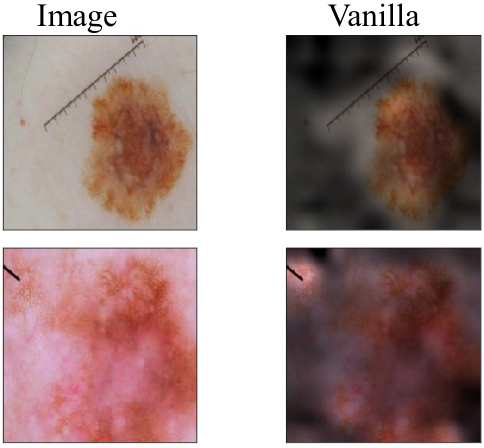
\includegraphics[width=0.6\textwidth]{./images/interps-are-useful-saliency-maps.png}
    \caption{Cutout of Figure S6 from \cite{interps-are-useful}. Original description: \textit{
        Both networks learnt that proportionally more images with malignant lesions feature a ruler next to the lesion. To make
        comparison easier, we visualize the heatmap by multiplying it with the image. Visible regions are important for classification
    }}
    \label{fig:interps-are-useful-saliency-maps}
\end{figure}
\pagebreak

\chapter{Theory}
This report assumes that the reader is familiar with the basics of machine learning.
This includes basic linear algebra, data preprocessing and model selection.
Further, understanding of how neural networks function is assumed,
including the basic concept of gradient descent used for model training.

The theory described in this section is what is directly relevant to the analysis.
Some concepts that are not directly used in analysis,
but needed to understand parts of the theoretical background,
have been moved to Appendix \ref{sec:background-theory}.
The chosen theory is focused on the parts used for explainable AI, more than the technical details of how neural networks work.
In addition, a small introduction to the domain knowledge of skin lesion diagnosis is given.

\section{Lesions of the skin}
Skin lesions are parts of the skin,
that have abnormal amounts of growth compared to the surrounding skin \cite{dermatologi-laerebogen}.
In medical science, they categorize these into subcategories,
that can be treated in different ways.
Such a category can be considered \texit{malignant} or \texit{benign}.
A malignant lesion is cancerous and thus a lot more dangerous than the non-cancerous benign ones. 
The most common type of malignant lesion is \texit{melanoma}. 
In practice some lesions might be classified as \textit{pre-malignant},
like the Bowen's disease,
that is cancerous but easily treatable \cite{nhs-bowens-disease}.

Using a skin biopsy,
a doctor can precisely identify the type of a lesion.
This is done by removing a small skin sample and looking at it under a microscope.

Due to the time and cost of the biopsy,
a pre-evaluation of a lesion is needed to determine if it is likely to be malignant.
Doctors use methods like the ABCD method,
that is looking at Asymmetry, Border irregularity, Color variation and Diameter ($>6\text{mm}$)\cite{dermatologi-laerebogen}.
It is this presevaluation process that a computer can be used to help doctors spend less time,
by trying to make a prediction only based on an image of the lesion.

\subsection{Classification problems}\label{sec:classification-problems}
The classification problem as a data scientist can therefore be either the binary classification problem,
where the model is trying to predict if a lesion is benign or malignant.
For these binary problems, we will consider pre-malignant lesions as malignant,
as we in a medical context would like a doctor to be aware that treatment is necessary.

It can also be the multi-class classification problem,
where the model is attempting to predict the exact kind of a lesion.
Both of these are discussed in this report.

\section{Model metrics} \label{sec:model_metrics}
To compare the performance of models, different kinds of metrics can be used.
As mentioned in Section \ref{sec:classification-problems},
researchers tackle two different kinds of classifications.
To enable comparison with as many other studies as possible,
we will report different metrics
on both problems as described in the following.
All of the metrics are in the $\[0, 1\]$ interval with $0$ being the worst score and $1$ being the best.

\subsection{Multi-class Accuracy}
Accuracy is the percentage of predictions that are correct.
\[
    \text{Accuracy} = \frac{\text{correct classifications}}{\text{total predictions}}
\]
Accuracy as a metric is not that good for problems with big class imbalance,
such as this one where a single class accounts for more than half of the data,
which is the case in the HAM10000 dataset that is used in this report (see Table \ref{table:ham10000}).

\subsection{Binary Accuracy}
The binary accuracy is defined exactly as the multi-class, but except of using all classes,
the considered classes are just benign and malignant.
Obviously, that means what $\text{Binary Accuracy} > \text{Multi-class Accuracy}$.

\subsection{Malignant recall}
The general definition of recall in a binary classification problem is the percentage of the positive class
that is correctly classified.
The recall is defined as
\[
    \text{Recall} = \frac{\text{TP}}{\text{TP} + \text{FN}}
\]
Here $TP$ is the number of true positives, and $FN$ is the number of false negatives.
When referring to \textit{malignant recall}, we will think of the recall metric in the problem
where the considered classes are just benign and malignant.
As the name suggest, the positive class is malignant.

An intuitive way of thinking about this is how big a portion of the malignant lesions
that the model was able to detect.
On its own, a very high malignant recall does not mean the model is excellent,
as one can trivially, make it $1$ by just having a model that always predicts malignant, no matter the image.

\subsection{Malignant F1 score}
For the binary \textit{malignant vs. benign} problem, we would like to have a general score 
that takes class imbalance into account.
For this purpose, the F1 score is often used.
In general, the F1 score is defined as
\[
    \text{F1 score} = \frac{2 \cdot \text{Precision} \cdot \text{Recall}}{\text{Precision} + \text{Recall}}
\]
giving rise to the need of for positive class, as the definition of recall requires one.
Here, the \textit{Malignant F1 score} is defined as
\[
    \text{Malignant F1 score} = \frac{2\cdot \text{Precision} \cdot \text{Malignant recall}}{\text{Precision} + \text{Malignant recall}}
\]

A benefit of the F1 score is that it is a good metric to compare the performance of different models,
as it both takes the class imbalance into account,
but also just the general performance of the model.

Malignant recall is usually referred to as \texit{sensisivity} in medical literature
\cite{sensitivity-and-specificity}.

\subsection{Multi-class F1 score}
Defining a multi-class F1 score, is a bit more complicated than for a binary one.
The Python package that is used to calculate the F1 score in this project, \verb|sklearn|
\cite{sklearn}, has a mandatory parameter \verb|average|, that changes the way the F1 score is calculated.
In Figure \ref{fig:sklearn-f1-average-docs} the average parameter is described.
In this project, we will use \verb|average='weighted'|, where the F1 score is calculated
individually for each class in the problem as a positive class,
and then doing a weighted average of them based
on the number of samples in each class.
The reason for this choice,
is that it explicitly considers the class imbalance,
which is important for the multi-class problem on the HAM10000.


\begin{center}
    \begin{minted}{text}
    average : {'micro', 'macro', 'samples','weighted', 'binary'} or None, \
            default='binary'
        This parameter is required for multi-class/multi-label targets.
        If ``None``, the scores for each class are returned. Otherwise, this
        determines the type of averaging performed on the data:

        ``'binary'``:
            Only report results for the class specified by ``pos_label``.
            This is applicable only if targets (``y_{true,pred}``) are binary.
        ``'micro'``:
            Calculate metrics globally by counting the total true positives,
            false negatives and false positives.
        ``'macro'``:
            Calculate metrics for each label, and find their unweighted
            mean.  This does not take label imbalance into account.
        ``'weighted'``:
            Calculate metrics for each label, and find their average weighted
            by support (the number of true instances for each label). This
            alters 'macro' to account for label imbalance; it can result in an
            F-score that is not between precision and recall.
        ``'samples'``:
            Calculate metrics for each instance, and find their average (only
            meaningful for multilabel classification where this differs from
            :func:`accuracy_score`).
    \end{minted}
    \captionof{figure}[Cutout from sklearn documentation for F1 score]{
        Documentation for the required \textit{average} parameter for the F1 score in a multi-class problem
        (Copied from \url{https://scikit-learn.org/stable/modules/generated/sklearn.metrics.f1_score.html
        })}
    \label{fig:sklearn-f1-average-docs}
\end{center}

\section{Saliency maps}\label{sec:saliency_maps}
When training deep neural networks,
it is difficult to know exactly what the model is doing.
Especially in fields like medical image analysis,
where the classification of a model might influence if a patient is correctly diagnosed or not,
it is very desirable to know what the model is doing to be able to critique its predictions.

In image analysis, a tool to try to understand models are the so-called \textit{saliency maps}.
A saliency map is supposed to be a visual representation of what parts of the image are influential on the model,
when it made a given prediction.
In Figure \ref{fig:interps-are-useful-saliency-maps} a saliency map over a skin lesion is shown. 

For instance, in a model supposed to classify if a picture of a bone is broken or not,
it is desirable that the model looks at the bone and not really, anything else in the image.

Many methods exist to produce saliency maps, each with their own strengths and weaknesses.
One of the most popular ones is the gradient-based method (explained below).
This method is popular because it is computationally efficient,
and the implementation comes almost for free if back propagation is implemented.

\subsection{Class specific gradient-based saliency maps} \label{sec:gradiant_saliency_maps}
As described in Section \ref{sec:partial_derivatives_of_scalar_over_vector},
if a function $f: \mathbb{R}^n \rightarrow \mathbb{R}$ is defined,
then the gradient of $f$ in a point $x\in\mathbb{R}$ is a vector in the space $\mathbb{R}^n$.
A special case of this, is where $f$ is an image classification model, that takes
an image (images can be vectorized, so we can consider them vectors) and returns a vector of probabilities for
different classes.
Then the gradient in any probability of the output vector, will be of the same size as the input vector.
Since the input vector was an image, the gradient can also be interpreted as an image.
It is this property that is utilized when calculating gradient-based saliency maps.

Often, these gradients are used as heatmaps over the image to highlight regions that
supposedly contributed a lot to the classification decision of the model.
For instance, in the book Interpretable Machine Learning (chapter 10.2)\cite{interpretable-machine-learning}, the gradient-based
saliency map method is described to
''assign each pixel a value that can be interpreted as the relevance of the pixel to the prediction or classification of that image''.
We should, however, be careful with that interpretation, as the gradient is just pointing to/away from the classification boundary.
Recent research is pointing toward problems with the usage of saliency maps as explained in the quote before\cite{false-hope}.
In the analysis, we will also see that the interpretations of these saliency maps are not always straightforward.

\section{The ResNet architecture}
The ResNet architecture is a popular architecture for deep neural networks.
It was presented in 2015 and showed some promising results on the ImageNet dataset\cite{RESNET-paper}.
The main idea in the architecture is to let some of the output from the internal convolutional layers
be \textit{fed forward} to layers a few layers deeper in the network.
The network is shown in Figure \ref{fig:resnet-18-architecture},
and the arrows show where the feed forward is happening.

\begin{center}
    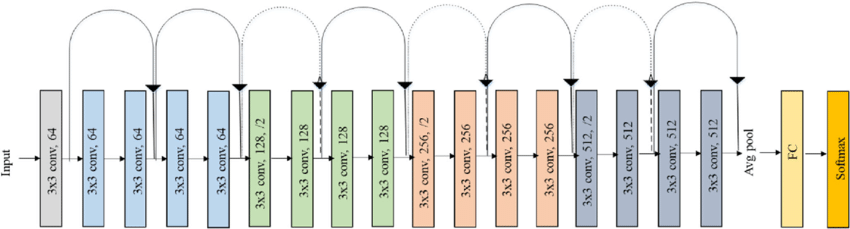
\includegraphics[width=0.9\textwidth]{images/ResNet-18-architecture.png}
    \captionof{figure}{ResNet-18 architecture. Figure taken from \cite{paper-with-resnet-18-figure}.
        The FC is short for Fully Connected layers, and the conv is short for convolutional layers. }
    \label{fig:resnet-18-architecture}
\end{center}


The architecture is implemented PyTorch\cite{PyTorch} and other similar libraries, making it easy to use.

\chapter{Model}
The initial goal of this project was to look into methods to not use ruler presence in the
diagnosis classification.
To be able to do this, a model that was using the ruler presence in its predictions was needed.
Preferably this model should also perform close to the best performing model, to be comparable.

\section{ResNet18 architecture trained with MixUp}
On the Kaggle classification competetion related to the HAM10000 dataset\cite{HAM10000-kaggle-competetion},
another user claimed to get a $97.7\%$ accuracy using a ResNet18 model trained with MixUp\cite{kaggle-97-model}.
When the provided model was retrained, the results were not as good as claimed.
The actual accuracy was in the range of $90\%$ to $92\%$, depending on the data split.
That is however still close to the best performing model published (see \ref{sec:state-of-the-art}).

The actual implementation of the model can be seen in Appendix \ref{appendix:resnet-18-mixup}.
Using the slight modifications to the original mode, the model reached an accuracy of roughly $91\%$.

\subsection{Model analysis}
\subsubsection{Prediction saliency map}
As described in the Introduction section, there is an academically described risk,
that the model will use the presence of rulers in its predictions. % Maybe a reference here?

We will first test this, by creating saliency maps (\ref{sec:saliency_maps}) for some of the images with rulers in the dataset.
These can be seen in Figure \ref{fig:ruler_saliency_map}.
More similar examples can be seen in Appendix \ref{appendix:ruler_saliency_maps}.

\begin{figure}[h]
    \includegraphics[
        width=\textwidth,
        height=\textheight,
        keepaspectratio=true,
        angle=0,
        clip=false
    ]{build/saliency_maps/overview_map_2.png}
    \caption{Saliency maps of the model prediction on an image with a ruler.}
    \label{fig:ruler_saliency_map}
\end{figure}

\subsubsection{Prediction precision on different classes}
To further evaluate the model, we will investigate wether it underperforms on some classes.
In Figure \ref{fig:prediction_strength} a confusion matrix for the trained model is shown.

\begin{figure}[ht]
    \centering
    \includegraphics[
        width=0.7\textwidth,
    ]{build/prediction_strength/confusion_matrix_seaborn.png}
    \caption{Confusion matrix of the model prediction on the dataset. 
        Normalization has been done over the truth.
    }
    \label{fig:prediction_strength}
\end{figure}

The confusion matrix shows that the model underperforms on the \verb|mel| (melanoma) class.
For terms of the using this model in practice, this would be problematic and should be adressed.
The model does however perform fairly well in general, so it will still be used to investigate the
impact of confounding elements on its predictions.

\subsubsection{Prediction strength on the melanoma class}
Assuming that the rulers do indeed affect the models predictions,
it would likely impact the prediction strength of the model if rulers are present. 
Since the rulers are overly present in the images of lesions with melanoma,
it would under the assumption be expected, that the presence of the rulers improves the model's predictions 
on the \verb|mel| class.

To test this, a plot has been created below that shows the prediction strength of the model on the \verb|mel| class,
seperated over the presence of rulers.

\begin{figure}
    \centering
    \begin{subfigure}[h]{0.45\textwidth}
        \includegraphics[
            width=\textwidth,
        ]{
            build/prediction_strength/mel_confusion_matrix_seaborn.png
        }
        \caption{No normalization}
        \label{fig:prediction_strength_mel}
    \end{subfigure}
    \begin{subfigure}[h]{0.45\textwidth}
        \includegraphics[
            width=\textwidth,
        ]{
            build/prediction_strength/mel_confusion_matrix_seaborn_normalized.png
        }
        \caption{Normalized over the presence of rulers}
        \label{fig:prediction_strength_mel_normalized}
    \end{subfigure}
    \caption{Confusion matrix of the model prediction the melanoma cases split up by presence of a ruler.}
\end{figure}


\end{figure}


\chapter{Experiments and Analysis}\label{sec:testing-the-hypothesis}
From both the background literature and general worry about models,
there is reason to believe that a model trained on the HAM10000 dataset will be biased
towards looking at confounding elements - hereunder the rulers in the image.
In the following, this hypothesis will be tested using both methods that other researchers have used,
and also other methods checking the output of the model.

\section{Prediction saliency map}\label{sec:prediction-saliency-map}
In \textit{Interpretations are useful: Penalizing Explanations to Align Neural Networks with Prior Knowledge}\cite{interps-are-useful},
(described in Section \ref{sec:interps-are-useful}), it is shown that a model trained on skin lesion images,
will mark out the ruler on malignant images containing one.
With the ResNet model described in \ref{sec:model}, similar saliency maps are constructed.

The saliency maps made here are gradient-based, as described in Section \ref{sec:gradiant_saliency_maps}.
In Figure \ref{fig:ruler_saliency_map} these can be seen.
More similar examples can be seen in Appendix \ref{appendix:ruler_saliency_maps}.

\begin{center}
    \includegraphics[
        width=\textwidth,
        height=\textheight,
        keepaspectratio=true,
        angle=0,
        clip=false
    ]{build/saliency_maps/overview_map_5.png}
    \captionof{figure}[Saliency maps of the model prediction on an image with a ruler.]{Saliency maps of the model prediction on an image with a ruler.
        The overlay on the right is the saliency map with a maximum filter and a uniform filter,
        stretched to the 0 to 1 range, multiplied elementwise onto the original image.
    }
    \label{fig:ruler_saliency_map}
\end{center}

\section{Feature based nearest neighbors}
In \textit{(De)biasing Skin Lesions Datasets and Model. Not so Fast}\cite{debias-not-so-fast} (described in Section \ref{sec:debias-not-so-fast}),
the authors argue that their melanoma prediction can pick up on confounding elements (like rulers),
by examining the internal layers of their model and comparing them to one another.
Specifically, they find, that the vectors outputted from internal layers,
that are thought of as representing the semantic features of an image,
have a short euclidean distance to one another.
For a detailed description, see section \ref{sec:debias-not-so-fast}.

To check if this is the case for our model, we use the same approach and make a similar plot as seen in Figure \ref{fig:not-so-fast-artifact-query}.

\begin{center}
    \includegraphics*[width=\textwidth]{build/near_neigh/examples.png}
    \captionof{figure}{Queries like the ones in Figure \ref{fig:not-so-fast-artifact-query} made for my own model
        All queries contain a ruler, and the neighbors have noted if they contain a ruler.
    }
    \label{fig:my-artifact-query}
\end{center}

Looking at Figure \ref{fig:my-artifact-query} we can see, that the results do not
suggest anywhere near as strong a correlation as the paper shows in Figure \ref{fig:not-so-fast-artifact-query}.
There does seem to be some amount more rulers than a random sample of images.
Whether that is necessarily due to the model being able to detect the rulers will be discussed later.

These images don't show results nearly as clearly as the ones from the article.
Where the paper had results showing the ruler clearly 0 these images will often just show a half of it.

\section{Statistical tests}\label{sec:statistical-tests}
Since the tests, described in the background literature, don't show clear evidence,
that the model is biased towards looking at rulers, we will also do some basic statistical tests,
to see if the model output is statistically significantly impacted by rulers.
All tests will be performed under the assumption that the model is indeed impacted by ruler presence.

\subsection{Different performance on the melanoma class?}\label{sec:different-performance-on-the-melanoma-class}
The confusion matrix in Figure \ref{fig:prediction_strength} shows that the model underperforms on the \verb|mel| (melanoma) class.
Since the rulers are overly present in the images of lesions with melanoma,
it seems likely that the presence of the rulers improves the model's predictions
on the \verb|mel| class.

To test this, a plot has been created below that shows the prediction strength of the model on the \verb|mel| class,
separated over the presence of rulers (Figure \ref{fig:prediction_strength_mel}).

It shows a slightly better melanoma prediction precision on the pictures with rulers (Figure \ref{fig:prediction_strength_mel_normalized}).
Doing a $\chi^2$ test on the data from Figure \ref{fig:prediction_strength_mel_not_normalized},
however, shows that the difference is not significant ($p=\input{build/prediction_strength/p_mel.txt}$).


\begin{center}
    \begin{subfigure}[h]{0.45\textwidth}
        \includegraphics[
            width=\textwidth,
        ]{
            build/prediction_strength/mel_confusion_matrix_seaborn.png
        }
        \caption{No normalization}
        \label{fig:prediction_strength_mel_not_normalized}
    \end{subfigure}
    \begin{subfigure}[h]{0.45\textwidth}
        \includegraphics[
            width=\textwidth,
        ]{
            build/prediction_strength/mel_confusion_matrix_seaborn_normalized.png
        }
        \caption{Normalized over the presence of rulers}
        \label{fig:prediction_strength_mel_normalized}
    \end{subfigure}
    \captionof{figure}{Confusion matrix of the model prediction on the melanoma cases split up by presence of a ruler.}
    \label{fig:prediction_strength_mel}
\end{center}

\subsection{Different performance on images containing rulers?}
If the rulers contribute to the model's predictions,
then the model might have a general better/worse performance on images containing them.
To investigate this claim, a plot like the one in Figure \ref{fig:prediction_strength_mel} has been made,
where just Correct/Incorrect predictions are separated over the presence of rulers.

\begin{figure}
    \centering
    \begin{subfigure}[h]{0.45\textwidth}
        \includegraphics[
            width=\textwidth,
        ]{
            build/prediction_strength/ruler_confusion_matrix_seaborn.png
        }
        \caption{No normalization}
        \label{fig:prediction_strength_ruler_not_normalized}
    \end{subfigure}
    \begin{subfigure}[h]{0.45\textwidth}
        \includegraphics[
            width=\textwidth,
        ]{
            build/prediction_strength/ruler_confusion_matrix_seaborn_normalized.png
        }
        \caption{Normalized over the presence of rulers}
        \label{fig:prediction_strength_ruler_normalized}
    \end{subfigure}
    \caption{Confusion matrix of the model prediction the cases split up by presence of a ruler.}
    \label{fig:prediction_strength_ruler}
\end{figure}

This plot tells a different story, than the one on just the \verb|mel| class.
The likelihood of a falsely classified image is almost twice as high for images
that contain a ruler.
Doing a $\chi^2$ test on the data from the confusion matrix in Figure \ref{fig:prediction_strength_ruler_not_normalized},
shows a significant difference ($p=\input{build/prediction_strength/p_ruler.txt}$).

\subsubsection{Controlling for classes}
From Figure \ref{fig:prediction_strength_ruler} and the following statistical test,
it became clear that there is a significant difference between performance on images containing rulers,
and on images without rulers.
As has been repeated in many a statistics course, though:
\textit{Correlation is not causation}.
That is, it is not necessarily \textit{because} of the rulers that the predictions are worse.
An explanation that would align with the results of Section \ref{sec:different-performance-on-the-melanoma-class},
could be that the model just has a more difficult time predicting the less prevalent malignant classes.
To test this, we need to control for the malignancy of the lesion in the image.

\paragraph{Malignant only}
On Figure \ref{fig:prediction_strength_ruler_malignant} yet another set of tables are set up,
comparing precision of the algorithm on the malignant subset of the test set.
It is slightly better at classifying the malignant cases, but not
significantly so under a $\chi^2$ test ($p=\input{build/prediction_strength/p_malignant.txt}$).

\begin{figure}[h]
    \centering
    \begin{subfigure}[h]{0.45\textwidth}
        \includegraphics[
            width=\textwidth,
        ]{
            build/prediction_strength/malignant_confusion_matrix_seaborn.png
        }
        \caption{Not normalized}
        \label{fig:prediction_strength_ruler_malignant_not_normalized}\
    \end{subfigure}
    \begin{subfigure}[h]{0.45\textwidth}
        \includegraphics[
            width=\textwidth,
        ]{
            build/prediction_strength/malignant_confusion_matrix_seaborn_normalized.png
        }
        \caption{Normalized over the presence of rulers and malignancy}
        \label{fig:prediction_strength_ruler_normalized_malignant}
    \end{subfigure}
    \caption{Confusion matrix of the model prediction based only on images of malignant lesions.}
    \label{fig:prediction_strength_ruler_malignant}
\end{figure}


\paragraph{Benign only}
On Figure \ref{fig:prediction_strength_ruler_benign} the same calculations have been made,
with the benign lesions, as were just made with the malignant ones.
They seem to show the opposite picture, where the images containing rulers are roughly
twice as likely to be incorrectly classified.
Testing with a $\chi^2$ test, this result is even statistically significant with
$p=\input{build/prediction_strength/p_benign.txt}$.

\begin{figure}[h]
    \centering
    \begin{subfigure}[h]{0.45\textwidth}
        \includegraphics[
            width=\textwidth,
        ]{
            build/prediction_strength/benign_confusion_matrix_seaborn.png
        }
        \caption{Not normalized}
        \label{fig:prediction_strength_ruler_benign}
    \end{subfigure}
    \begin{subfigure}[h]{0.45\textwidth}
        \includegraphics[
            width=\textwidth,
        ]{
            build/prediction_strength/benign_confusion_matrix_seaborn_normalized.png
        }
        \caption{Normalized over the presence of rulers and malignancy}
        \label{fig:prediction_strength_ruler_normalized_benign}
    \end{subfigure}
    \caption{Confusion matrix of the model prediction based only on images of benign lesions.}
\end{figure}

So, the algorithm is significantly worse at classifying benign lesions if they contain a ruler.
Again, this does not mean that it is because of the rulers, only that there is correlation.
A possible explanation could also be that other confounding elements are more present in images with rulers.
In Figure \ref{fig:prediction_strength_ruler_misclassified_benign} a sample of the misclassified images are shown,
and a lot of these contain other confounding elements like ink and black borders.
Due to the lack of data on the other confounders, no further exploration into these correlations has been done.

\begin{figure}
    \centering
    \includegraphics*[width=\textwidth]{
        build/prediction_strength/misclassified_benign_images_with_rulers.png
    }
    \caption{Misclassified benign lesions with rulers}
    \label{fig:prediction_strength_ruler_misclassified_benign}
\end{figure}

\section{Segmenting the lesion}
A widely used strategy for preventing a model use confounding information, is to simply remove it from the image.
In this case, that would mean to make the entire image black except the skin lesion.
Training another model on this data, would mean that it didn't have access to the confounding elements,
and will therefore be unable to learn about them.
On Figure \ref{fig:segmented_images_example} a sample of the images that have been segmented,
can be seen.

\begin{figure}[h]
    \centering
    \includegraphics*[width=\textwidth]{
        build/segmented_images_example/segmented_images_example.png
    }
    \caption{Examples of segmented lesions. The originals are shown above their segmented versions.}
    \label{fig:segmented_images_example}
\end{figure}

Operating under the assumption that the model is learning about confounding elements,
a worse performance would be expected from a model trained on a segmented dataset,
since it can't get the assumed advantage from looking at the confounding elements.

\begin{table}
    \input{build/segmented_prediction_strength/score_table.tex}
    \caption[Model metrics for model trained on both full and segmented images]{
        Model metrics for the two models on the model trained on both full and segmented images,
        then evaluated on each of the two for calculating metric.
        The reported metrics are defined in Section \ref{sec:model_metrics}.
    }
    \label{tab:segmented_metrics}
\end{table}

The most notable thing in Table \ref{tab:segmented_metrics} is that the segmented model tested
on its segmented images outperforms everything else on all metrics.
This finding has already been reported previously \cite{segmenting-improves-performance}.
The segmented model even outperforms the model trained on the full images, on the full images in Malignant recall.

\subsection{Saliency maps from model trained on segmented dataset}
Some saliency maps from Section \ref{sec:prediction-saliency-map},
are quite hard to interpret.
To have something to compare to, similar maps have been generated for the model
trained on the segmented dataset.
On Figure \ref{fig:segmented_prediction_saliency_map} an example of a classified lesion is shown.
All the same examples from \ref{sec:prediction-saliency-map} can be seen in Appendix \ref{appendix:ruler_saliency_maps}.
Interestingly, the segmented model seems to highlight the ruler at least as much, if not more than the non-segmented one.
\begin{figure}[ht]
    \centering
    \includegraphics*[width=\textwidth]{
        build/only_lesion_saliency_maps/overview_map_6.png
    }
    \caption{Saliency map of the model trained on the segmented dataset.}
    \label{fig:segmented_prediction_saliency_map}
\end{figure}

\chapter{Discussion}
Biases on models from confounding elements have been widely reported in machine learning
\cite{DeConstructing_Bias_on_Skin_Lesion_Datasets_2019, Towards_Explainable_Classifiers_Using_the_Counterfactual_Approach_2019, debias-not-so-fast, interps-are-useful}.

The initial goal of this project was to look into methods to not use ruler presence in the
classification of lesions.
To be able to investigate the phenomenon, the plan was to:
\begin{enumerate}
    \item Train a model that performs fairly well compared to the state of the art \label{item:train-model}
    \item Show that the model is using the presence of ruler in its predictions \label{item:biased-ruler}
    \item Make changes to the model to remove the bias
    \item Rerun the argument as in step \ref{item:biased-ruler} and show that the model is no longer biased
\end{enumerate}
Step \ref{item:train-model} went fairly easy, especially because the dataset is well researched,
so another model could be used for inspiration \cite{kaggle-97-model}.

When reaching step \ref{item:biased-ruler}, the results didn't go quite as expected.
Even though it had been argued in previous papers, that models were doing exactly this
\cite{debias-not-so-fast,interps-are-useful}, I was unable to replicate their results,
to a degree that convinced me that the model was indeed using the rulers.
This changed the focus of the project from removing biased predictions to instead investigating
if there were any biases at all.
In the following, we will go through the experiments made in Section \ref{sec:testing-the-hypothesis} and
examine the results in this light: Do they seem to indicate that the model is using the rulers?

The discussion will be divided into a part where the results of the analysis in Section \ref{sec:testing-the-hypothesis}
are examined, and a part where we will discuss the results of the project in its entirety.
It will be finished up with what obvious further research that could be done following up this project.

\section{Discussion of analysis}
\subsection{Saliency maps}
In Section \ref{sec:prediction-saliency-map} we investigated the saliency maps of the model predictions.
Previously other researchers had shown that the rulers would be indicated clearly on these maps \cite{interps-are-useful}.
Going through the same experiment with the model trained in this project, we found saliency maps that were
did not indicate anything very clearly. 
(see Figure \ref{fig:interps-are-useful-saliency-maps} and \ref{fig:ruler_saliency_map}).
In some instances, the saliency map was not even visible in the hightligthed areas,
and in others it was but not in a way where it was obviously using that specific element of the image.

In general saliency maps are very prone to confirmation bias \cite{sanity-checks-for-saliency,Grns2020FaithfulSM}.
It is nothing more than the gradient on a very complicated function.
Conclude that just because the ruler is sometimes highlighted partly on the saliency map,
it must mean that the model is using it, seems like a stretch on its own.
Especially when considering the saliency maps from the model trained on segmented images (Figure 
\ref{fig:segmented_prediction_saliency_map}) that is hightlighting the ruler to at least the same degree 
that the model trained on the entire dataset is.
We know for sure, that the model trained on the segmented dataset is not using the rulers,
as it has never seen a ruler during training.
It is unclear exactly what knowledge can be extracted from the saliency maps,
but using them to conclude that the model is using the rulers doesn't seem to be holding up.

We could have used different kinds of saliency maps, if we wanted to go further into the understanding 
the model in this way.
Due to the risk of confirmation bias mentioned earlier, we instead used the time on other approaches.

\subsection{Feature vector similarity}
The authors of \cite{debias-not-so-fast} also argued that their model was using rulers
and other confounding elements in its predictions.
Their argument was based rougly around the idea that if the extracted features from two images
containing rulers are more similar to each other than the rest of the dataset, then the model is using them.

The first problem with using that approach in this report, is that the results didn't replicate.
Where the auther of \cite{debias-not-so-fast} showed that finding the nearest neighbors in the feature
vector space would all contain rulers, we only saw roughly half of them containing ruler 
(See their result on Figure \ref{fig:not-so-fast-artifact-query} and ours on Figure \ref{fig:my-artifact-query}).

Another problem, is that even if the results had contained more images with rulers,
it might not even have been the case that the model was even aware of them.
We have already shown, that the rulers correlate with the true diagnosis of the lesions (see Figure \ref{fig:ruler_vs_dx}).
Since the model is trained to predict the true diagnosis, we would expect them to have similar feature vectors.
What we see could therefore be the model finding other lesions that have similar diagnosis,
and therefore are also most likely to have rulers.

Even if images with rulers actually \textit{had} similar feature vectors \textit{because} of the rulers,
it would still not neccessarily be the case that the model was using them.
The architecture used in the model is pretrained on another big image dataset,
so a lot of the features that is extracted are not relevant to the final classification. 
The final fully connected layers of the model are in charge of extracting the relevant features.
So to use this method, we would also need to weight the features after how relevant they are to
the final classification.
That could for instance be done by running the backpropagation algorithm and see the
gradient in each of the features of the vector and weight by them in the distance metric.

\subsection{Statistical analysis of model predictions}
To investigate if the model was using the rulers in its predictions, 
we ran quite a few statistical tests (Section \ref{sec:statistical-tests}).
In most of the tests, we weren't able to identify that the model was biased.
In a few cases, we were able to identify statistically significant correlation between
the models prediction and the presence of rulers.
All of these related to the prediction strength of the model on images.
The points can be rougly summarized as:
\begin{enumerate}
    \item The model was worse at predicting the class of images that contained a ruler
    \item The model was worse at predicting the class of images of benign lesions where a ruler was present 
    \item The model was not significantly worse at predicting the class of malignant lesions if a ruler was present
\end{enumerate}

A tempting conclusion from a researcher looking into if a model is biased or not,
is that the model is classifying the benign lesions as malignant due to the ruler indicating them 
as malignant.
Another explanation could also be, that the rulers are simply present in benign images that are 
difficult to classify.
When a doctor decides to place a ruler next to a lesion,
it is due to a concern that the lesion is malignant.
If a benign lesion has a ruler, then it seems that the doctor found 
some aspect of the lesion that makes worried her, 
hence the lesion is probably more difficult to classify.

\section{Discussion of project}
\subsection{Does the Clever Hans phenomenon even exist?}
All of these arguments arguing that the model are probably influenced by the presence of rulers,
could seem like we are arguing that the Clever Hans phenomenon doesn't exist.
That is not at all the case, the phenomenon definetly exists.
Of course litterature can be found on the topic, but I also encountered it during the project.
I tried to train a classifier just for the rulers, and I ended up with a classifier that would
be decent at classifying the lesion instead. 
In Figure \ref{fig:ruler_classifier_saliency_map} a saliency map of the ruler classifiers prediction is shown,
where it clearly is using the lesion and not the ruler.

\begin{center}
    % Taken from this message: https://slackers-k4k1590.slack.com/archives/C0301E3TZ6J/p1645645248107699
    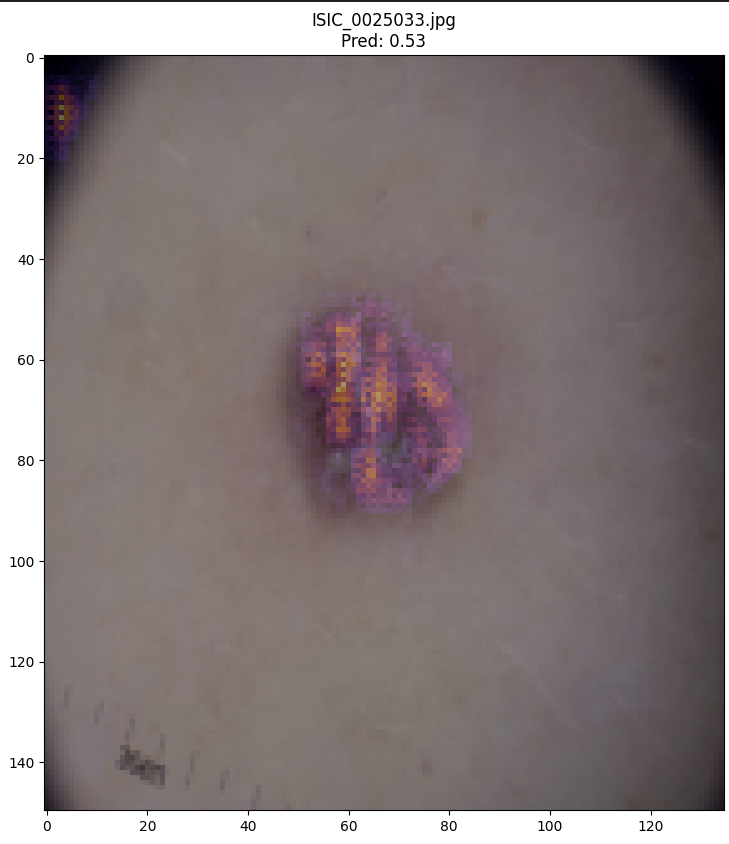
\includegraphics[width=0.5\textwidth]{images/ruler_classifier_saliency.png}
    \captionof{figure}{Saliency map from a ruler classifier that I trained during the project.}
    \label{fig:ruler_classifier_saliency_map}
\end{center}

This clearly shows the Clever Hans phenomenon in action.
To make it work, the model had to be quite poor - in this case the model didn't have a lot of layers,
and was only trained on a small subset of the dataset.

So the Clever Hans phenomenon is very real, but just because it could occur, doesn't mean that it will in all cases.

\subsection{Are no models affected by the rulers?}
As mentioned multiple times, multiple other researches have been convinced that the models that 
they trained were using the rulers.
It is impossible for us to verify without access to their model.
There is a possibility that the model trained in this project is simply better in some way making it not use the rulers.
I am however critical of that theory, though I cannot refute it completely.
During the project, I trained many different models of varying architectures,
and in none of them I was able to find clear cut evidence that the model was using the rulers.
Even though I tried, making my models biased was difficult, 
so for someone to train a model by mistake that is seems unlikely - but of course not impossible.

\subsection{How big of an impact can be expected from confounfing elements?}
% Those introduced by humans can never be better than what a human can predict
% That of course depends largely on how the dataset is assembled.
% Also mention the point about it can't be that big, since it performs hella well
% on the segmented images.


\subsection{Why are these results even relevant?}



\section{Further research}


\chapter{Conclusion}
The work done in this project shows that a model trained on the HAM10000 
dataset is likely not affected by the fact that rulers are present significantly
more in images of malignant lesions than in images of benign ones.
This statement is checked using experiments used by other researchers in the field
to conclude that their models are using the rulers in its predictions.

The results and discussion shows how difficult it can be to understand what
exactly, deep neural networks are doing.
At the same time it shows why it is crucial to control what information we feed
to our model, as figuring out what parts of it are used is very difficult.

How difficult it was to check if the model was using the rulers in its predictions
also show that researchers have to be cautious when concluding that a model
they have trained is or isn't using some part of the provided information.

\pagebreak
\listoffigures
\listoftables

\pagebreak
\printbibliography[title={Litterature}]
\pagebreak
% Start the appendix
\appendix
\part{Appendix}
\chapter{Background theory}\label{sec:background-theory}

\section{Tensors}\label{sec:tensor}
The following definitions and concepts are heavily based on \textit{Introduction to Convolutional Neural Networks} by J. Wu \cite{tensorIntroduction}.
In linear algebra, the concept of a vector is introduced.
Further a 2-dimensional vector is introduced, the \textit{matrix}.
We will denote a vector as $\vecsym{v}\in \mathbb{F}^n$ and a matrix as $\matsym{M}\in \mathbb{F}^{m\times n}$.
Here $\mathbb{F}$ is a field.
For the purpose of this report, a field can be considered a set of element with a defined addition and multiplication operation.
Especially most of the time the field will be the real numbers, $\mathbb{R}$.

Having defined vectors and matrices, we can now define a tensor as the natural extension of the matrix abstraction,
by adding more dimensions.
A $3$-dimensional tensor is can then be defined as $\tenssym{T}\in \mathbb{F}^{m\times n\times c}$.
Such a tensor is a natural way to represent an image in colors.
Such a representation of an image of height $h$ and width $w$ could then be represented as an
element in $\mathbb{F}^{h\times w\times 3}$.

An example of a higher order tensor used in this project, could be a batch of images.
Such a batch could be represented as a tensor of shape $(h, w, c, b)$ where $b$ is the batch size.
That is, the entire batch would be a $4$-dimensional tensor in the tensor-space $\mathbb{F}^{h\times w\times c\times b}$.

\subsection{Vectorizing tensors}
As noted in most introductions of linear algebra, matrices are themselves vectors.
This is to be understood as, any matrix $\matsym{M} \in \mathbb{F}^{m\times n}$ can be represented as a vector $\vecsym{m} \in \mathbb{F}^{m\cdot n}$.
This is commonly done by stacing the columns of the matrix, e.g.  if
\begin{equation}
    \matsym{M} = \begin{bmatrix}
        m_1 & m_2 & m_3 \\
        m_4 & m_5 & m_6 \\
        m_7 & m_8 & m_9
    \end{bmatrix} \in \mathbb{F}^{3 \times 3}
\end{equation}
then the vector representation is
\begin{equation}
    \vecsym{m} = \begin{bmatrix}
        m_1 & m_4 & m_7 & m_2 & m_5 & m_8 & m_3 & m_6 & m_9
    \end{bmatrix}^T \in \mathbb{F}^{9}
\end{equation}
The same concept can be applied to tensors of higher dimensions than the $2$-dimensional matrix,
by stacking the columns continously.

\subsection{Partial derivatives over vectors} \label{sec:partial_derivatives_of_scalar_over_vector}
In multiple setings in training of neural networks, it is neccesarry to figure out what
parts of the model contributed to the result of the model.
During training, we for instance want to know what parts of the model contributed to an increase of the loss function,
so that these parts can be changed thereby hopefully improving the model.
In this report it is also used for creating saliency maps, and discussing them (see section \ref{sec:gradiant_saliency_maps}).

Defining the partial derivative of a vector $\vecsym{v}\in\mathbb{F}^n$ with respect to a scalar $s$ is done as follows:
\begin{equation}
    \left[ \frac{\partial s}{\partial \vecsym{v}} \right]_i
    = \frac{\partial s}{\partial \vecsym{v}_i}
\end{equation}

Note that with this definition, derivatives over matrices can also be done by first vectorizing them,
and we then get the nice algebraic property that  $\frac{\partial s}{\partial \vecsym{v}}^{T} = \frac{\partial s}{\partial \vecsym{v}^{T}}$


\subsection{Partially deriving vector functions}
Suppose $\vecsym{x} \in \mathbb{F}^n$,
$f: \mathbb{F}^n \rightarrow \mathbb{F}^m$ and
$\vecsym{y} = f(\vecsym{x}) \in \mathbb{F}^m$.
Then
\begin{equation}
    \left[ \frac{\partial \vecsym{y}}{\partial \vecsym{x}^T} \right]_{ij} =
    \frac{\partial \vecsym{y}_i}{\partial \vecsym{x}_j}
\end{equation}

Which means that the derivative of a vector function on the form of $f$ will be a matrix/$2$-tensor
in the tensor-space $\mathbb{F}^{m\times n}$.


\section{Convolutional neural networks (CCNs)} \label{sec:convolutional_neural_networks}
Convolutional neural networks (CNNs) are a fairly modern method used in image classification.
They are based on the idea of a convolutional layer, which is a way of combining pixels in a
neighbourhood of an image into single features.

The mathemathical basis is the \textit{convolution} of a matrix.
During the definition of convolutions, the following matrix will be used as an example:
\begin{equation}
    \matsym{I} = \input{build/convolution_example/I.tex}
\end{equation}

Think of $\matsym{I}$ as an image.
Sematically there is an area in the \"image\" that has way higher values than the rest
(the lower right corner).
A convolution on the image, will reduce this information to a more compact representation.
To do this, a matrix kernel needs to be defined. It's standard to use a square kernel.
Here we will use a $3 \times 3$ kernel:
\begin{equation}
    \matsym{K} =
    \input{build/convolution_example/K.tex}
\end{equation}

To then convolve $\matsym{I}$ with $\matsym{K}$, we \textit{move} the kernel over the image,
and multiply each index of the kernel with the index that it is currently \textit{above} in the image
(a full mathemathical deifintion follows lates in section \ref{sec:convolution_definition}).
That will in this case result in the matrix:
\begin{equation}
    \input{build/convolution_example/convolution.tex}
\end{equation}


On Figure \ref{fig:convolution_example} heatmaps of the original $I$ and the convolved, shows that they look very similar.
\begin{figure}[h]
    \centering
    \begin{subfigure}{0.45\textwidth}
        \includegraphics[width=\textwidth]{build/convolution_example/I.png}
        \caption{Original version of $I$}
    \end{subfigure}
    \begin{subfigure}{0.45\textwidth}
        \includegraphics[width=\textwidth]{build/convolution_example/convolution.png}
        \caption{Convolution of $I$ with $K$}
    \end{subfigure}
    \caption{Heatmaps of the original $I$ and the convolved $I$}
    \label{fig:convolution_example}
\end{figure}

Comparing the heatmaps on Figure \ref{fig:convolution_example}, makes it clear that little to no imformation about
where the high values are in the picture has been lost.
The amount of data points has however been reduced.

\subsection{Padding}
The current model of moving the kernel over the image, will not prioritize the borders
of the image a lot.
To compat this, the image is often padded - usually with zeros.
This is done by adding a border of zeros around the image, the width of which is referred to as the size of the padding.
By default, the padding in libaries like PyTorch \cite{PyTorch} is $0$ (no padding) as in the example before.

To continue the example, we will now use a padding of $1$ around the image.
\begin{equation}
    \matsym{I}_{\text{padded}} = \input{build/convolution_example/I_padded.tex}
\end{equation}

Calculating the convolution of the padded image with the kernel, results in the following matrix:
\begin{equation}
    \input{build/convolution_example/convolution_padded.tex}
\end{equation}

And again plotting the heatmaps we see two similar images again:
\begin{figure}[h]
    \centering
    \begin{subfigure}{0.45\textwidth}
        \includegraphics[width=\textwidth]{build/convolution_example/I.png}
        \caption{The original $\matsym{I}$}
    \end{subfigure}
    \begin{subfigure}{0.45\textwidth}
        \includegraphics[width=\textwidth]{build/convolution_example/convolution_padded.png}
        \caption{Convolution of $\matsym{I}_{\text{padded}}$ with $K$}
    \end{subfigure}
    \caption{Heatmaps of the padded $\matsym{I}_{\text{padded}}$ and the convolved $\matsym{I}_{\text{padded}}$}
    \label{fig:convolution_example_padded}
\end{figure}

Note that padding increases the amount of data points in the image, but that
the effect of this is not as extreme as it seems in the example, since images a usually
a lot larger than this small example.

\subsection{Stride}
To reduce the amount of data points even further, we can use a stride.
This is done by moving the kernel over the image as before, but moving multiple pixelse each time.

Following the example from before using a stride of $2$ and a padding of $1$, the convolution results in the following matrix:
\begin{equation}
    \input{build/convolution_example/convolution_stride.tex}
\end{equation}

This is again plotted in Figure \ref{fig:convolution_example_stride}.

\begin{figure}[ht]
    \centering
    \begin{subfigure}{0.45\textwidth}
        \includegraphics[width=\textwidth]{build/convolution_example/I.png}
        \caption{The original $\matsym{I}$}
    \end{subfigure}
    \begin{subfigure}{0.45\textwidth}
        \includegraphics[width=\textwidth]{build/convolution_example/convolution_stride.png}
        \caption{Convolution of $\matsym{I}_{\text{padded}}$ with stride $2$}
    \end{subfigure}
    \caption{Heatmaps of the original $\matsym{I}$ and the convolved $\matsym{I}_{\text{padded}}$}
    \label{fig:convolution_example_stride}
\end{figure}

It is again clear that the data seems similar to the original image, but the data points
has been reduced from $\input{build/convolution_example/I_size.tex}$ to $\input{build/convolution_example/final_convolution_size.tex}$.

In convolutions can combine information from data where some kind of \textit{proximity} is important.
This is very much the case in image analysis (hence the focus in this explanation), but the idea is
not limited to this field.

\subsubsection{Full definition of convolutions}\label{sec:convolution_definition}
The above is a very simple example of a convolution.
A full compact formula for making a convolution is left out, as it is not readable and
ultimately not very insightful.
Instead we will make a implementation of the a \verb|convolve| function in Python.
To define such an algorithm, it is usefull to know the output size of the final matrix.
Let the width of the original image be $w$, the kernel size be $k$, the padding be $p$, and the stride be $s$.
Calculating the output width can then be done by finding all the possible values of $w$ that can be
used as the left value of the kernel.
First the padded size of the image is seen to be $w + 2p$.
Since a kernel is moved over the picture, the last $k-1$ pixels cant be used to place a kernel.
Assuming that the image is non-empty and the kernel is smaller than or the same size as the image,
at least one kernel can be placed, adding up to a total of $k$ pixels where a kernel cannot be placed.
Of the remaining only $1/s$ of the pixels are actually used to place a kernel, hence the output width becomes:
\begin{equation}
    w_{out} = \left\lfloor \frac{w + 2p - k}{s}\right\rfloor + 1
\end{equation}

And with a completely similar procedure for the height, $h$, we get:
\begin{equation}
    h_{out} = \left\lfloor \frac{h + 2p - k}{s} \right\rfloor + 1
\end{equation}

Having these values, we can then define a Python function that performs the convolution:

\inputminted[]{python}{src/convolve.py}

\section{The power of convolution kernels}
In the example in Section \ref{sec:convolutional_neural_networks}, a convolution that
comprimed the image into a condensed version was used.

Kernels can do lot more than compressing images though.
For the following, different types of kernels are used to convolute an image of a Model of the Greek Temple of Artemis \cite{greek-temple-picture}.

With a kernel like this:
\begin{equation}
    K_{\text{edge}} = \input{build/kernel_examples/K_edge.txt}
\end{equation}
an image is produced where the edges are highlighted.

\begin{figure}[ht]
    \centering
    \begin{subfigure}{0.45\textwidth}
        \includegraphics[width=\textwidth]{build/kernel_examples/image_scaled.jpg}
        \caption{The original image}
    \end{subfigure}
    \begin{subfigure}{0.45\textwidth}
        \includegraphics[width=\textwidth]{build/kernel_examples/edges.jpg}
        \caption{The image considered as a matrix convolved with $K_{\text{edge}}$}
    \end{subfigure}
    \caption{The image with the edges highlighted}
\end{figure}

In a similar way, a kernel like this:
\begin{equation}
    K_{\text{vertical}} = \input{build/kernel_examples/K_vertical.txt}
\end{equation}
can be used to highlight the vertical lines in the image.

\begin{figure}[ht]
    \centering
    \begin{subfigure}{0.45\textwidth}
        \includegraphics[width=\textwidth]{build/kernel_examples/image_scaled.jpg}
        \caption{The original image}
    \end{subfigure}
    \begin{subfigure}{0.45\textwidth}
        \includegraphics[width=\textwidth]{build/kernel_examples/vertical.jpg}
        \caption{The image considered as a matrix convolved with $K_{\text{vertical}}$}
    \end{subfigure}
    \caption{The image with the vertical lines highlighted}
\end{figure}

A lot of other interesting kernels exist, see for instance these examples at AI Shack \cite{kernel-example-webpage}.

The point we want to make here, is that a lot of different information can be extracted from an image,
if the correct kernel is used.
When training a convolutional layer of a neural network, it is exactly the kernel values that optimized.

\section{Backpropagation}
The back propagation algorithm is a fundamental part of how we train a neural network.
As this report does not focus on the details of how deep learning works, we will only discuss the
basic structure of the algorithm and not the specific mathemathical details.

The purpose of the backpropagation algorithm is to find the gradient of the model parameters with respect
to some output of the model - most commonly the loss function.
That is, if some output of the model $z$ is produced, the backpropagation algorithm finds the gradient over
the internal weights of the neural network.

Consider a neural network consisting of $L$ layers and lett $\vecsym{w}^L$ be the weights in the $L$'th layer.
Then the backpropogation algorithm will find
$\frac{\partial z}{\partial \vecsym{w}^L}$ for each value of $L$.
For the purpose of model training where $z$ indicates the loss, updating each layer as
$\vecsym{w}^L \leftarrow \vecsym{w}^L - \eta \frac{\partial z}{\partial \vecsym{w}^L}$
is called gradient descent.
Note the $\eta$ parameter that is used to update the weights.
This is called the learning rate, since it determines how fast the weights are updated during training.

The obvious problem is then how $\frac{\partial z}{\partial \vecsym{w}^L}$ is calculated.
The specifics of how that works can be seen on page 9 of Introduction to Convolutional Neural Networks \cite{tensorIntroduction}.

\chapter{ResNet18 architecture trained with MixUp}\label{appendix:resnet-18-mixup}
This is very heavily inspired by the competetion Kaggle competetion submission by Leon Blume \cite{kaggle-97-model}.

The training was done on DTU high performance computing cluster\cite{dtu-hpc}.
Here a GPU was used, specifically the Tesla V100 16 GB.
\section{Model}
\inputminted{python}{models/resnet_mixup/ham10000_resnet.py}
\section{Output}
\inputminted{python}{models/resnet_mixup/pretty-Output}
\chapter{Ruler saliency maps}\label{appendix:ruler_saliency_maps}
\input{build/saliency_maps/saliency_maps_appendix.tex}
\end{document}